%
%===============>>  Сторожук Модуль 5 <<=============
%
\setmodule{5}

%BEGIN_FOLD % ====>>_____ Занятие 1 _____<<====
\begin{class}[number=1]
	
	\begin{listofex}
		\item   Занятие 1
	\end{listofex}
\end{class}
%END_FOLD

%BEGIN_FOLD % ====>>_____ Занятие 2 _____<<====
\begin{class}[number=2]
	\begin{listofex}
		\item Занятие 2
	\end{listofex}
\end{class}
%END_FOLD

%BEGIN_FOLD % ====>>_ Домашняя работа 1 _<<====
\begin{homework}[number=1]
	\begin{listofex}
		\item  Найти значения выражения:
		\begin{tasks}(2)
			\task \( 2^{\log_26-3} \)
			\task \( 7\cdot5^{\log_54} \)
			\task \( 6^{5\log_63} \)
			\task \( \log_2112-\log_27 \)
			\task \( \log_340,5+\log_36 \)
			\task \( 6^{3\log_62} \)
			\task \( \dfrac{\log_318}{2+\log_32} \)
			\task \( (\log_381)\cdot(\log_6216) \)
		\end{tasks}
		\item 	
			\begin{minipage}[t]{\bodywidth}
			На рисунке изображён график функции \[ f(x)=kx+b. \] Найдите \(f(-200)\).
		\end{minipage}
		\hspace{0.02\linewidth}
		\begin{minipage}[t]{\picwidth}
			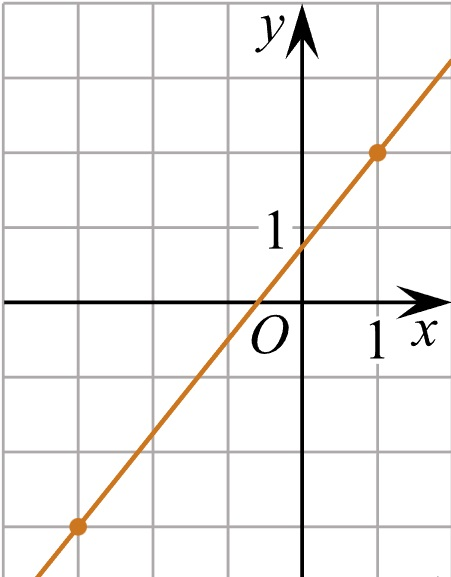
\includegraphics[align=t, width=\linewidth]{../../pics/G101M4C4-1}
		\end{minipage}
		\item 
		\begin{minipage}[t]{\bodywidth}
			На рисунке изображены графики функций \( f(x)=4x^2-25x+41 \) и \( g(x)=ax^2+bx+c \), которые пересекаются в точках \(A\) и \(B\). Найдите абсциссу  \( B \).
		\end{minipage}
		\begin{minipage}[t]{\picwidth}
			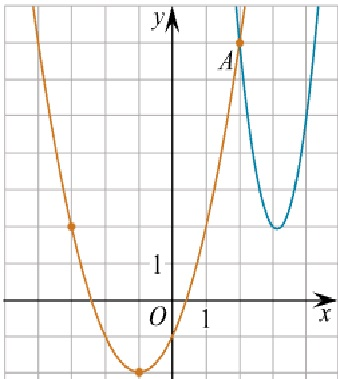
\includegraphics[align=t, width=\linewidth]{../../pics/G111M3PP-1}
		\end{minipage}
	\end{listofex}
\end{homework}
%END_FOLD

%BEGIN_FOLD % ====>>_____ Занятие 3 _____<<====
\begin{class}[number=3]
	\begin{listofex}
		\item Занятие 3
	\end{listofex}
\end{class}
%END_FOLD

%BEGIN_FOLD % ====>>_____ Занятие 4 _____<<====
\begin{class}[number=4]
	\begin{listofex}
		\item Занятие 4
	\end{listofex}
\end{class}
%END_FOLD

%BEGIN_FOLD % ====>>_ Домашняя работа 2 _<<====
\begin{homework}[number=2]
	\begin{listofex}
		\item ДЗ 2
	\end{listofex}
\end{homework}
%END_FOLD

%BEGIN_FOLD % ====>>_____ Занятие 5 _____<<====
\begin{class}[number=5]
	\begin{listofex}
		\item Занятие 5
	\end{listofex}
\end{class}
%END_FOLD

%BEGIN_FOLD % ====>>_____ Занятие 6 _____<<====
\begin{class}[number=6]
	\begin{listofex}
		\item Занятие 6
	\end{listofex}
\end{class}
%END_FOLD

%BEGIN_FOLD % ====>>_ Домашняя работа 3 _<<====
\begin{homework}[number=3]
	\begin{listofex}
		\item ДЗ 3
	\end{listofex}
\end{homework}
%END_FOLD

%BEGIN_FOLD % ====>>_____ Занятие 7 _____<<====
\begin{class}[number=7]
	\begin{listofex}
		\item \textit{Расширенное понятие синуса и косинуса:}\\[0.5em]
		\fbox{%
			\begin{minipage}[t]{0,4\textwidth}
				
				\textbf{\boldmath\( {\cos x} \)} --- абсцисса точки на единичной окружности, соответствующей углу \( x \).
				
				\textbf{\boldmath\( \sin x \)} --- ордината точки на единичной окружности, соответствующей углу \( x \).
			\end{minipage}
		}
	\item Вычислить: \quad \( \sin90\degree;\;\sin270\degree;\;\sin180\degree;\;\cos0\degree;\;\cos360\degree;\;\sin(-90\degree);\\
	\sin720\degree;\;\sin0\degree;\;\cos900\degree \)
	\item Выяснить, почему при \( n\in Z \):
	\begin{tasks}(2)
		\task \( \sin(x+360\degree\cdot n) = \sin x \);
		\task \( \cos(x+360\degree\cdot n) = \cos x \);
		\task \( \tg(x+360\degree\cdot n) = \tg x \);
		\task \( \ctg(x+360\degree\cdot n) = \ctg x \).
	\end{tasks}
	\item Доказать геометрическим способом, что:
	\begin{tasks}(2)
		\task \( \sin(-x) = -\sin x \);
		\task \( \cos(-x) = \cos x \).
		\task \( \sin(180 - x) = \sin x \);
		\task \( \cos(180 - x) = -\cos x \);
		\task \( \sin(180+x) = -\sin x \);
		\task \( \cos(180+x) = -\cos x \).
	\end{tasks}
	\item Вычислить:
	\begin{tasks}(5)
		\task \( \cos120\degree \)
		\task \( \cos150\degree \)
		\task \( \sin225\degree \)
		\task \( \sin(-135\degree )\)
		\task \( \cos225\degree \)
		\task \( \tg(-120\degree) \)
		\task \( \cos405\degree \)
		\task \( \sin540\degree \)
		\task \( \cos(-510\degree) \)
		\task \( \sin(-450\degree) \)
	\end{tasks}
		\item \textbf{Формулы суммы/разности синуса или косинуса:}
		\begin{tasks}(1)
			\task \( \sin(x+y)=\sin x\cos y + \sin y \cos x \)
			\task \( \sin(x-y)=\sin x\cos y - \sin y \cos x \)
			\task \( \cos(x+y)=\cos x \cos y - \sin x \sin y \)
			\task \( \cos(x-y)=\cos x \cos y + \sin x \sin y \)
		\end{tasks}
	\item Вычислить:
	\begin{tasks}(4)
		\task \( \sin 300\degree \)
		\task \( \cos 240\degree \)
		\task \( \tg 330\degree \)
		\task \( \cos 120\degree \)
		\task \( \sin 390\degree \)
		\task \( \cos 495\degree \)
		\task \( \cos (-780\degree) \)
		\task \( \sin (-300\degree) \)
		\task \( \tg (-225\degree) \)
		\task \( \sin (-1200\degree) \)
	\end{tasks}
	\end{listofex}
		\begin{definit}
		Радиан --- центральный угол, который опирается на дугу, равную радиусу данной окружности.
		\end{definit}
		\begin{definit}
		Число \( \pi \) --- отношение длины окружности к ее диаметру. Или иначе отношение половины длины окружности к ее радиусу.
		\end{definit}
		Таким образом можно сделать вывод, что в половине окружности радиус умещается \( \pi \) раз, а значит развернутый угол равен \( \pi \) радиан (т.е. \( \pi \) радиан \( = 180\degree \)).
		\begin{tasks}(1)
		\task \( 1 \) градус \( = \dfrac{\pi}{180} \) радиан;
		\task \( 1 \) радиан \( = \dfrac{180}{\pi}\) градусов (по факту всегда вместо \( \pi \) подставляем \( 180\degree \)).
		\end{tasks}
		\begin{listofex}[resume]
			\item Перевести радианы в градусы:
			\begin{enumcols}[itemcolumns=4]
				\item \( \dfrac{3\pi}{4} \)
				\item \( \dfrac{7\pi}{2} \)
				\item \( \dfrac{11\pi}{6} \)
				\item \( \dfrac{42\pi}{4} \)
			\end{enumcols}
			\item Перевести градусы в радианы:
			\begin{enumcols}[itemcolumns=4]
				\item \( 30\degree \)
				\item \( 11\degree \)
				\item \( 22,5\degree \)
				\item \( 225\degree \)
			\end{enumcols}
\end{listofex}
\end{class}
%END_FOLD

%BEGIN_FOLD % ====>>_ Занятие 8 _<<====
\begin{class}[number=8]
	\begin{listofex}
		\item \textbf{Метод приведения аргумента тригонометрических функций:}
	\begin{tasks}(1)
		\task Выносим минус за знак аргумента;
		\task "Убираем"{ }полные круги из аргумента \textit{(в будущем не обязательно);}
		\task Представляем аргумент в виде суммы/разности так, чтобы одно слагаемое было кратно \( 90 \), а другое было табличным значением (\( 30\degree;\;45\degree;\;60\degree \));
		\task Определяем четверть аргумента \textit{(меньшее слагаемое всегда принимаем за острый угол);}
		\task Определяем знак функции в этой четверти;
		\task Меняем или оставляем название тригонометрической функции (\( 0\degree;\;180\degree \) --- не меняем название функции; \( 90\degree;\;270\degree \) --- меняем название функции на противоположное).
	\end{tasks}
	\item Вычислить с помощью метода приведения:
	\[ \sin135\degree;\;\cos240\degree;\;\sin390\degree;\;\tg150\degree;\;\ctg220\degree;\;\sin(-220\degree);\;\tg840\degree;\;\cos(-240\degree);\;\sin315\degree \]
	
		\item Вычислить с помощью метода приведения: \[ \sin150\degree;\;\cos135\degree;\;\sin225\degree;\;\cos(-120\degree);\;\cos330\degree;\;\tg(-150\degree);\;\sin(-225\degree);\;\cos300\degree;\;\sin(-315\degree) \]
		\item Вычислить с помощью метода приведения:
		\[ \cos\dfrac{5\pi}{4};\;\sin\dfrac{7\pi}{3};\;\sin\dfrac{3\pi}{2};\;\sin\left( -\dfrac{5\pi}{3} \right);\;\cos\dfrac{7\pi}{6};\;\sin\dfrac{13\pi}{4};\;\sin\left( -\dfrac{7\pi}{6}  \right);\;\cos\dfrac{21\pi}{4} \]
		\item Вычислить:
		\begin{tasks}(1)
			\task \( \dfrac{\sqrt{3}}{\sin60\degree}+\dfrac{3}{\sin30\degree} \)
			\task \( \dfrac{17\sin155\degree}{\sin25\degree} \)
			\task \( \dfrac{-2\sin105\degree}{\cos15\degree} \)
			\task \( \sin^215\degree-1+\cos^215 \)
			\task \( -\sqrt{27}\cos30\degree-\sqrt{2}\sin45\degree\ctg60\degree\tg60\degree\)
			\task \( \dfrac{9\sin45\degree\cos45\degree}{\cos^245\degree-\sin^245\degree} \)
		\end{tasks}
	\end{listofex}
\end{class}
%END_FOLD